\documentclass[pdflatex,compress,mathserif]{beamer}

%\usetheme[dark,framenumber,totalframenumber]{ElektroITK}
\usetheme[darktitle,framenumber,totalframenumber]{ElektroITK}

\usepackage[utf8]{inputenc}
\usepackage[T1]{fontenc}
\usepackage{lmodern}
\usepackage[bahasai]{babel}
\usepackage{amsmath}
\usepackage{amsfonts}
\usepackage{amssymb}
\usepackage{graphicx}
\usepackage{multicol}

\newcommand*{\Scale}[2][4]{\scalebox{#1}{$#2$}}%

\title{PEMODELAN JARINGAN KOMUNIKASI}
\subtitle{Dynamic Host Configuration Protocol}

\author{Tim Dosen Pengampu}

\begin{document}
	
\maketitle

\section{DHCP Dynamic Host Configuration Protocol}


\begin{frame}
	\frametitle{DHCP – Dynamic Host Configuration Protocol}
	\begin{itemize}
		\item DHCP is a client/server protocol that automatically provides a host
with its IP address and other related configuration information such as
the subnet mask and default gateway.
		\item DHCP clients obtain their IP configuration information from a DHCP
server, rather than being manually configured.
	\end{itemize}
\end{frame}

\begin{frame}{DHCP – Dynamic Host Configuration Protocol}
	\begin{center}
		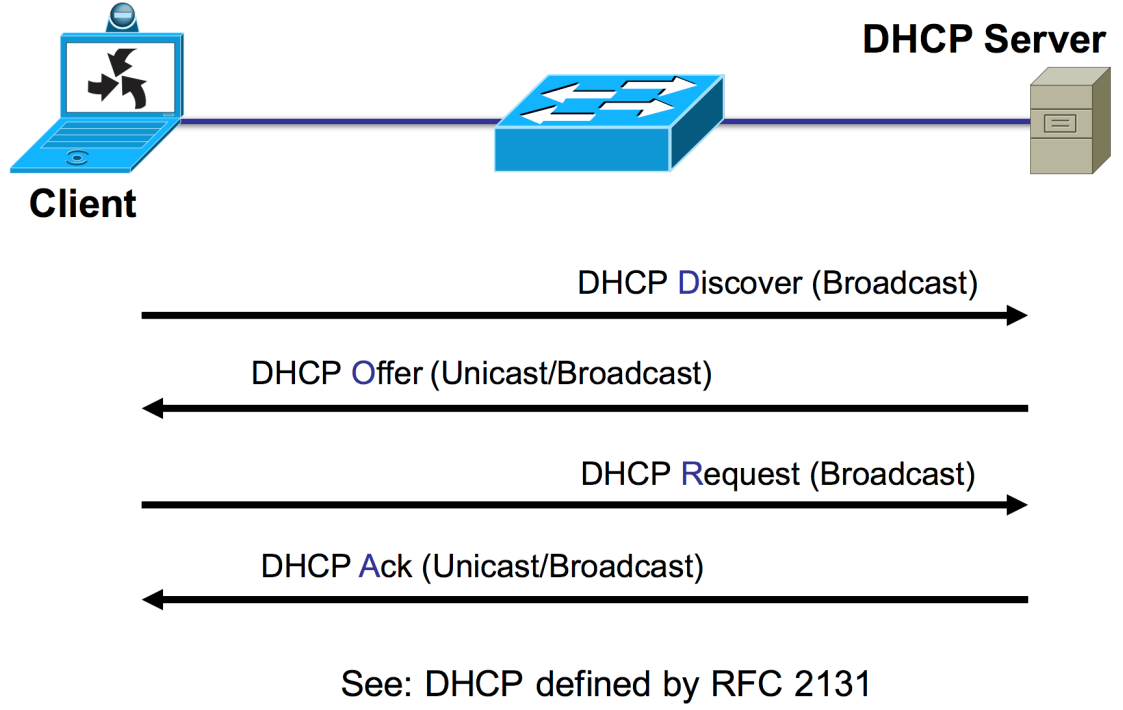
\includegraphics[width=0.8\linewidth]{img/img01}
	\end{center}
\end{frame}

\begin{frame}
	\frametitle{DHCP Benefits – Reduced Network Admin}
	\begin{itemize}
		\item Centralized and automated IP configuration, rather than manually
assigning an IP address to every host.
		\item Can assign additional IP configuration values by means of DHCP
options.
		\item Efficient handling of clients that must be updated frequently, such as
laptops that move to different locations on a wireless network.
		\item The forwarding of initial DHCP messages by using a DHCP relay agent,
which eliminates the need for a DHCP server on every subnet.
	\end{itemize}
\end{frame}

\begin{frame}
	\frametitle{DHCP Benefits - Reliable IP address configuration}
	\begin{itemize}
		\item DHCP minimizes configuration errors caused by manual IP address
configuration, such as typos, or address conflicts caused by the
assignment of an IP address to more than one computer at the same
time.
	\end{itemize}
\end{frame}

\begin{frame}
	\frametitle{DHCP Clients}
	\begin{itemize}
		\item Desktop PCs are good candidates to be DHCP clients because there will
typically be many of them in an office. Using DHCP saves a lot of admin
work that would be necessary if manually configuring IP addresses.
		\item They do not accept incoming connections so it does not matter if their
IP address changes.
	\end{itemize}
\end{frame}

\begin{frame}{DHCP Clients}
	\begin{itemize}
		\item Servers and network infrastructure devices such as routers and
switches will not typically be DHCP clients.
		\item They are mission critical devices which do not move and are required
for the network and its services to function.
		\item Their IP addresses are manually configured to ensure they will not
change and are not dependant on DHCP.
	\end{itemize}
\end{frame}

\section{Cisco DHCP Server}

\begin{frame}
	\frametitle{DHCP – Dynamic Host Configuration Protocol}
	\begin{itemize}
		\item DHCP is a client/server protocol that automatically provides a host
with its IP address and other related configuration information such as
the subnet mask and default gateway.
		\item DHCP clients obtain their IP configuration information from a DHCP
server, rather than being manually configured.
	\end{itemize}
\end{frame}

\begin{frame}{DHCP – Dynamic Host Configuration Protocol}
	\begin{center}
		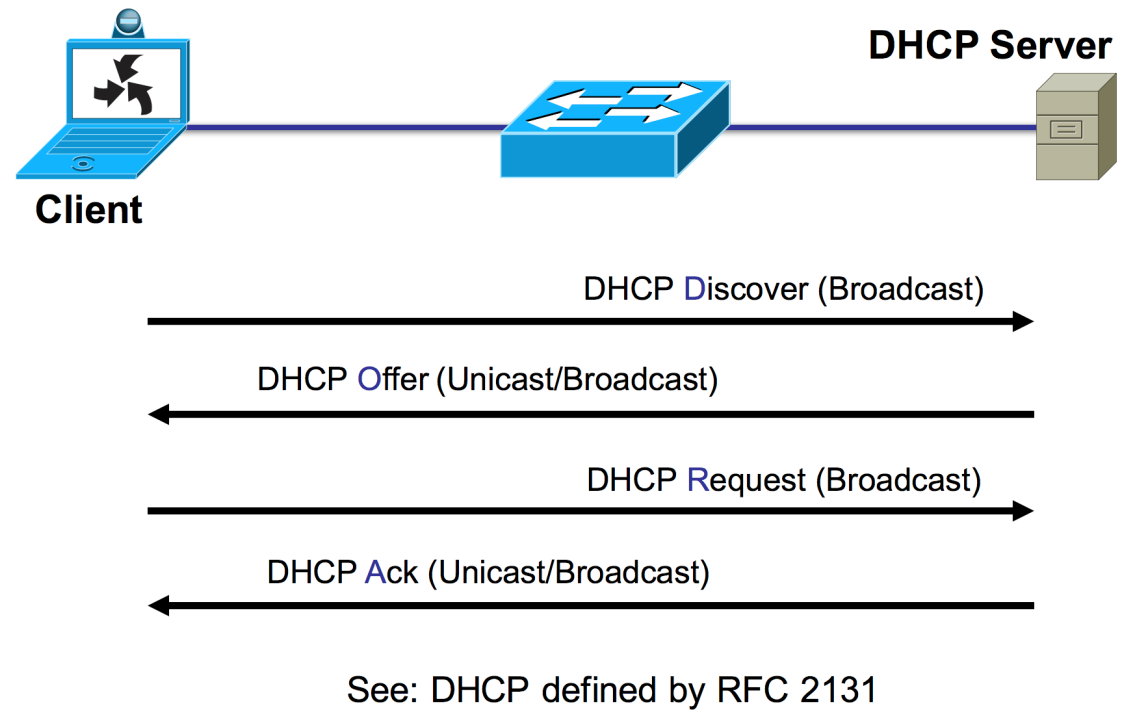
\includegraphics[width=0.8\linewidth]{img/img02}
	\end{center}
\end{frame}

\begin{frame}
	\frametitle{DHCP Benefits – Reduced Network Admin}
	\begin{itemize}
		\item Centralized and automated IP configuration, rather than manually
assigning an IP address to every host.
		\item Can assign additional IP configuration values by means of DHCP
options.
		\item Efficient handling of clients that must be updated frequently, such as
laptops that move to different locations on a wireless network.
		\item The forwarding of initial DHCP messages by using a DHCP relay agent,
which eliminates the need for a DHCP server on every subnet.
	\end{itemize}
\end{frame}

\begin{frame}
	\frametitle{DHCP Benefits - Reliable IP address configuration}
	\begin{itemize}
		\item DHCP minimizes configuration errors caused by manual IP address
configuration, such as typos, or address conflicts caused by the
assignment of an IP address to more than one computer at the same
time.
	\end{itemize}
\end{frame}

\begin{frame}
	\frametitle{DHCP Clients}
	\begin{itemize}
		\item Desktop PCs are good candidates to be DHCP clients because there will
typically be many of them in an office. Using DHCP saves a lot of admin
work that would be necessary if manually configuring IP addresses.
		\item They do not accept incoming connections so it does not matter if their
IP address changes.
	\end{itemize}
\end{frame}

\begin{frame}{DHCP Clients}
	\begin{itemize}
		\item Servers and network infrastructure devices such as routers and
switches will not typically be DHCP clients.
		\item They are mission critical devices which do not move and are required
for the network and its services to function.
		\item Their IP addresses are manually configured to ensure they will not
change and are not dependant on DHCP.
	\end{itemize}
\end{frame}

\begin{frame}
	\frametitle{Option 1: Cisco DHCP Server Configuration}
	\begin{center}
		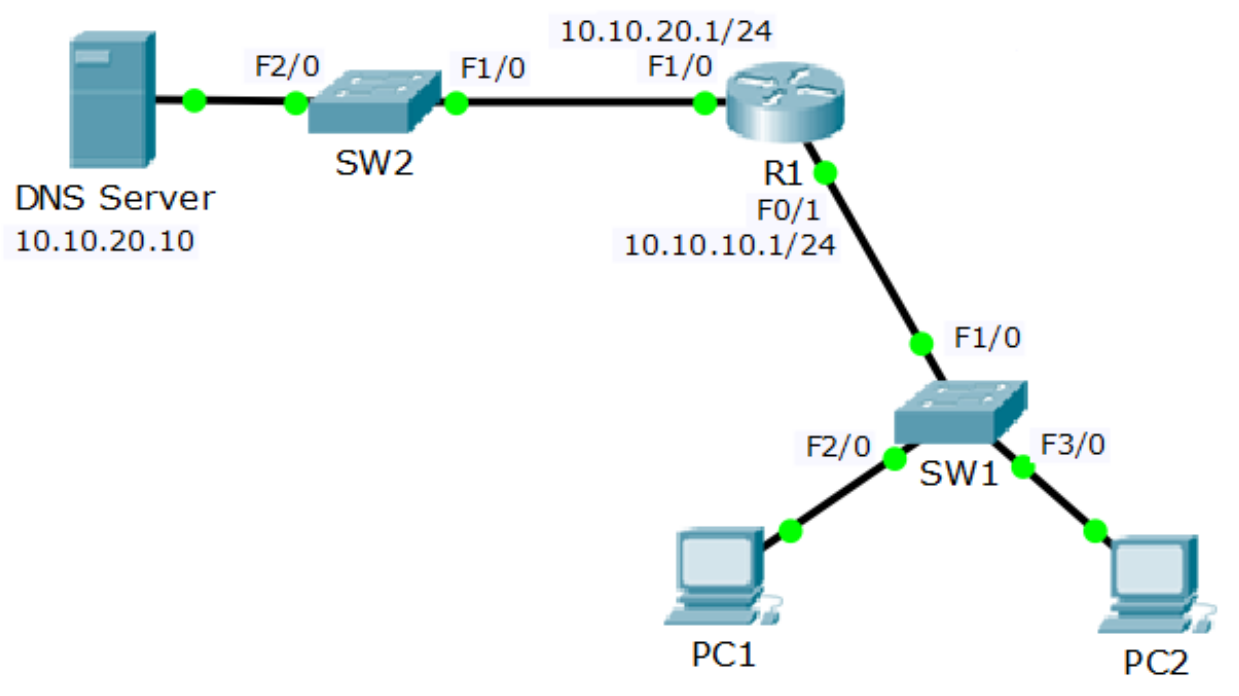
\includegraphics[width=0.8\linewidth]{img/img03}
	\end{center}
\end{frame}

\begin{frame}{Option 1: Cisco DHCP Server Configuration}
	\begin{center}
		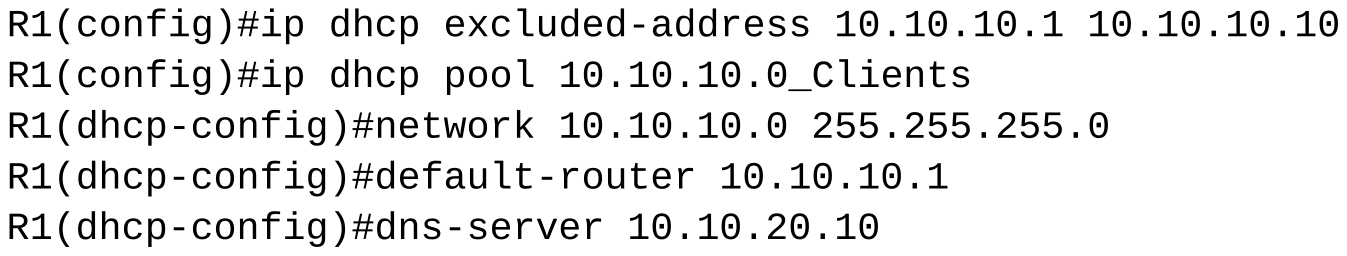
\includegraphics[width=0.8\linewidth]{img/img04}
	\end{center}
\end{frame}

\begin{frame}
	\frametitle{Verification – show ip dhcp pool}
	\begin{center}
		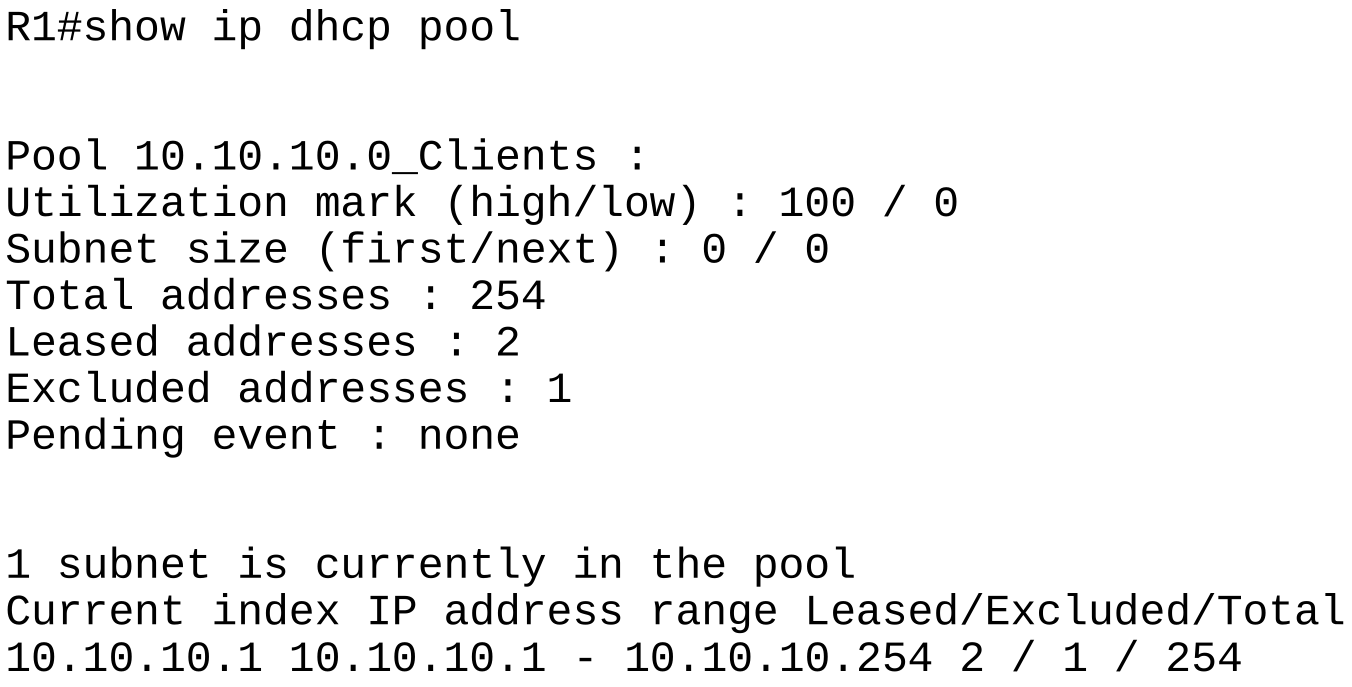
\includegraphics[width=\linewidth]{img/img05}
	\end{center}
\end{frame}

\begin{frame}
	\frametitle{Verification – show ip dhcp binding}
	\begin{center}
		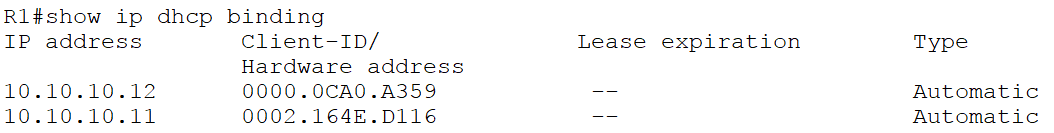
\includegraphics[width=\linewidth]{img/img06}
	\end{center}
\end{frame}

\begin{frame}
	\frametitle{Lab}
	\begin{center}
		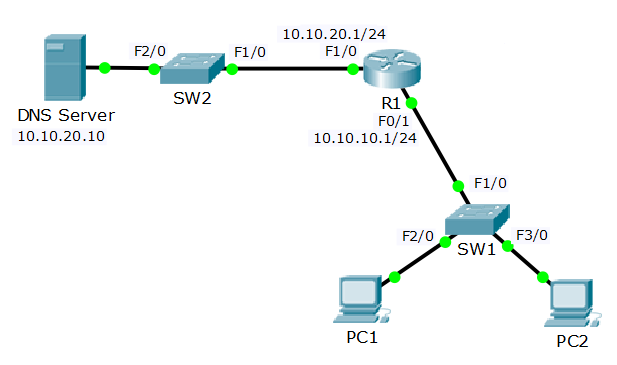
\includegraphics[width=\linewidth]{img/img07}
	\end{center}
\end{frame}

\section{External DHCP Server}

\begin{frame}
	\frametitle{Option 2: External DHCP Server Configuration}
	\begin{center}
		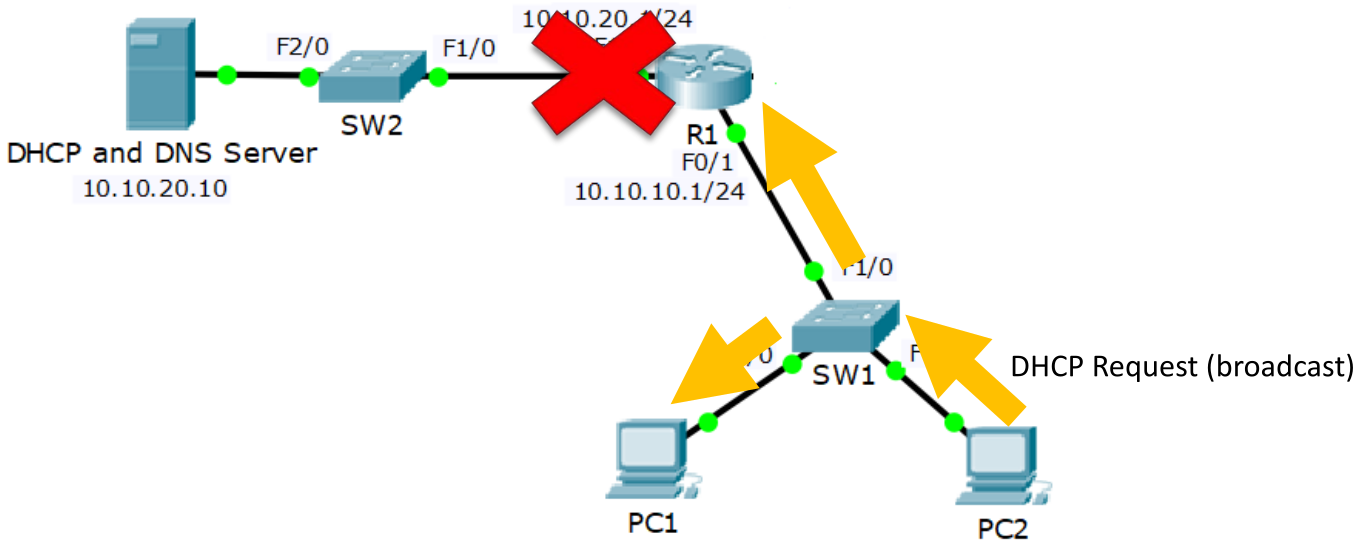
\includegraphics[width=\linewidth]{img/img08}
	\end{center}
\end{frame}

\begin{frame}{Option 2: External DHCP Server Configuration}
	\begin{center}
		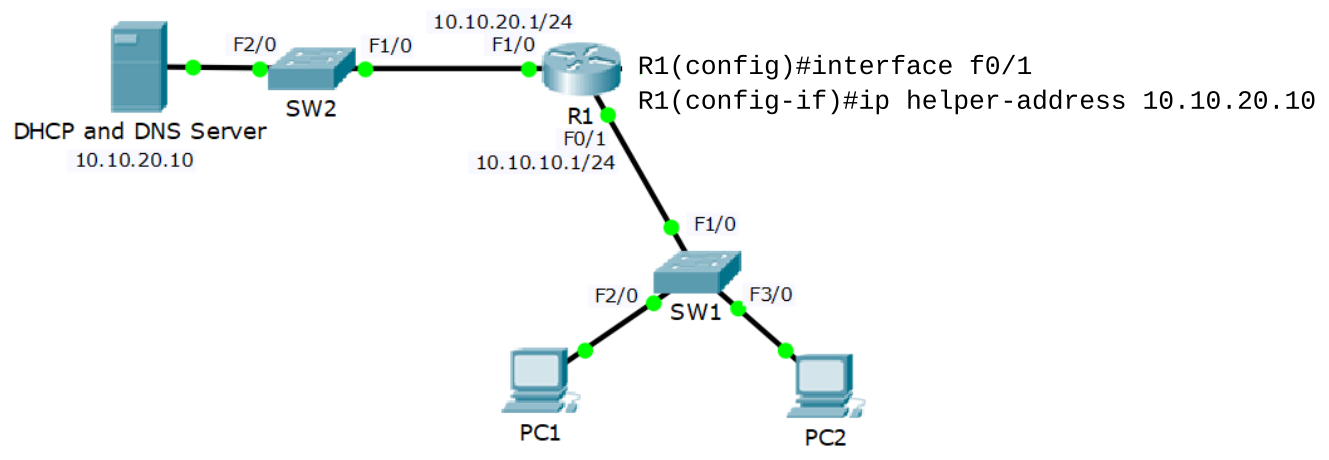
\includegraphics[width=\linewidth]{img/img09}
	\end{center}
\end{frame}

\section{Cisco DHCP Client}

\begin{frame}
	\frametitle{Configuring a Cisco Router as a DHCP Client}
	\begin{itemize}
		\item Cisco routers are typically manually configured with static IP addresses
		\item An exception to this is where an office is connected to the Internet but
has not bought static public IP addresses (because it does not contain
any publicly available servers which would need a fixed IP address for
incoming connections)
		\item The office still requires a public IP address to allow internal hosts
outbound connectivity to the Internet through NAT
		\item In this case the router will receive the public IP address on its outside
interface from the Internet service provider via DHCP
	\end{itemize}
\end{frame}

\begin{frame}{Configuring a Cisco Router as a DHCP Client}
	\begin{center}
		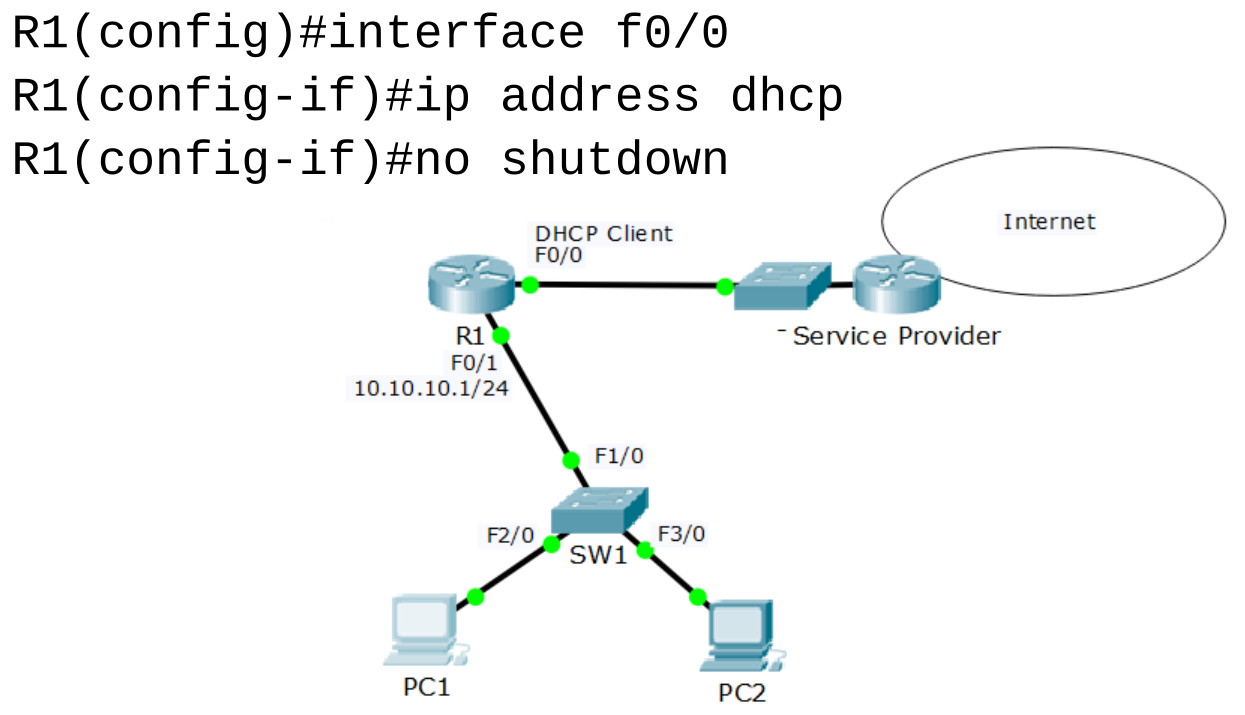
\includegraphics[width=\linewidth]{img/img10}
	\end{center}
\end{frame}

\begin{frame}
	\frametitle{Verification – show dhcp lease}
	\begin{center}
		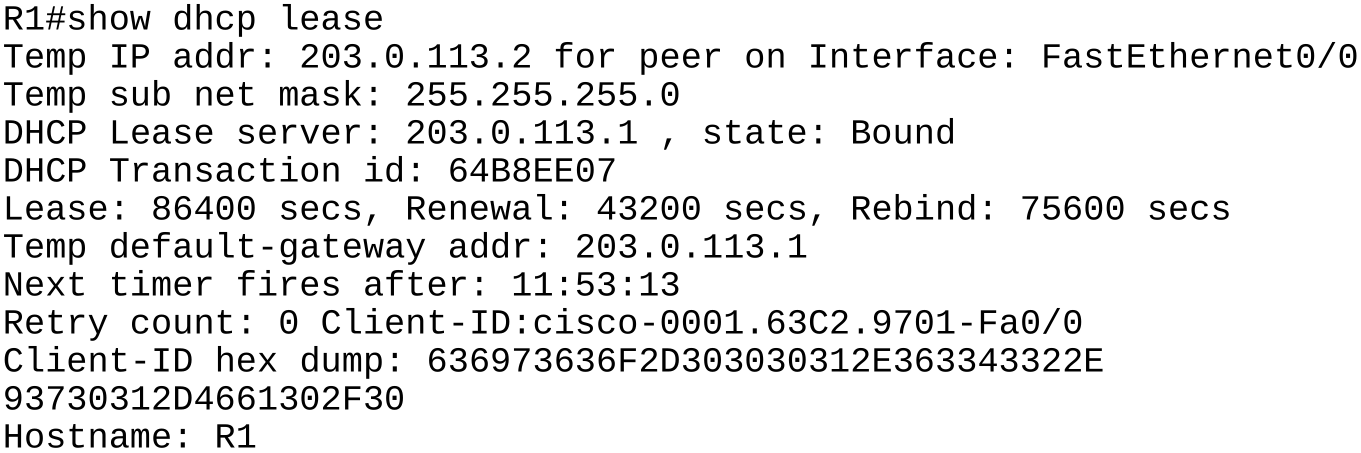
\includegraphics[width=\linewidth]{img/img11}
	\end{center}
\end{frame}

\end{document}